\section{Estudio de inversión, financiamiento y análisis financiero}

\subsection{Criterios de la proyección}

La evaluación financiera ayuda a comparar la inversión, los costos y los
ingresos para estudiar si un negocio puede sostenerse \parencite{baca2016}.
Para Pulso, el equipo elaboró un escenario financiero preliminar con un cliente
Starter y clientes Pro Gym posteriores. Los cálculos se presentan en las tablas
y gráficas de este informe. Son estimaciones propias que deberán revisarse con
cotizaciones, pruebas piloto y clientes reales.

Premium y Enterprise se reservan para una etapa posterior. Podrían incluir
diseño propio, atención dedicada y una base de datos independiente. Como aún
falta estimar el costo de cada caso, quedan fuera de esta proyección.

El análisis distingue el costo económico del dinero que entra y sale. El costo
económico incluye el valor de las horas del equipo, aunque no se paguen al
inicio. El flujo de efectivo registra los cobros y pagos previstos. Todos los
precios se expresan en colones.

\subsection{Inversión, recursos y financiamiento}

El trabajo de desarrollo pendiente se estima en CRC 198\,735,27. El equipo
aportaría esas horas sin cobrarlas al inicio, junto con computadoras, teléfonos
y conexión disponibles. Se propone una reserva inicial de CRC 40\,000 para
atender pagos. El proyecto aún no reporta préstamos, inversión externa ni
ingresos comerciales.

\begin{table}[htbp]
\caption{Recursos e inversión inicial de Pulso}
\begin{tabularx}{\textwidth}{>{\bfseries}p{3.8cm}r X}
\toprule
Concepto & CRC & Tratamiento \\
\midrule
Trabajo de desarrollo pendiente & 198\,735,27 & Costo económico aportado por el equipo; no desembolso inicial. \\
Reserva inicial propuesta & 40\,000 & Reserva de efectivo proyectada para iniciar la etapa comercial. \\
Equipo de desarrollo y pruebas & Aporte en especie & Computadoras, teléfonos, internet y herramientas disponibles. \\
Financiamiento externo & 0 & No se han declarado préstamos ni inversión de terceros. \\
\bottomrule
\end{tabularx}
\caption*{\textit{Nota}. Elaboración propia a partir del escenario financiero preliminar. Los aportes están previstos para el inicio del servicio.}
\end{table}

Antes de cobrar por el servicio se revisarán la forma de registrar el negocio,
las obligaciones tributarias y de seguridad social, los costos de los trámites
y la participación adulta necesaria. Mientras se resuelven estas condiciones,
las pruebas mantendrán carácter educativo
\parencite{codigo_comercio_cr,hacienda_rut,ccss_independiente}.

\subsection{Costos operativos y capacidad}

El presupuesto incluye infraestructura, viáticos, publicidad, correo, diseño,
mantenimiento, búsqueda de clientes, soporte, nube e instalación. La
base mensual de gastos fijos y trabajo valorado es CRC 114\,247,54; el costo
variable se ajusta conforme aumenta la cartera. El primer mes contempla un costo
de incorporación mayor que el de un mes de operación habitual.

Antes de operar se revisarán los impuestos, las comisiones bancarias, los
trámites y los gastos por consumos adicionales o problemas del servicio.
También se prepararán respaldos, almacenamiento y separación de información
para atender más de un gimnasio.

\subsection{Fuentes y condiciones del análisis de precios}
\label{sec:fuentes-precios}

Se contrastaron los servicios presupuestados con las páginas oficiales de sus
proveedores el 18 de septiembre de 2026. Las tarifas se expresan en dólares y
se convierten con el supuesto presupuestario de CRC 500 por USD. Esta tasa es
una decisión de planificación; no se presenta como cotización vigente del
Banco Central. Las promociones temporales no se usan para reducir el costo.

\begin{longtable}{p{3.1cm}p{4.0cm}p{6.8cm}}
\caption{Tarifas de referencia para los servicios tecnológicos}\\
\toprule Servicio & Tarifa publicada & Aplicación y condición \\
\midrule\endfirsthead
\toprule Servicio & Tarifa publicada & Aplicación y condición \\
\midrule\endhead
Vercel Pro & USD 20 al mes; CRC 10\,000. & Base de alojamiento. Incluye crédito de uso; consumos y puestos adicionales pueden generar cargos. No incluye impuestos \parencite{vercel_precios}. \\
Supabase Pro & Desde USD 25 al mes; CRC 12\,500. & Base de datos y servicios asociados. El costo aumenta según cómputo, proyectos y consumo \parencite{supabase_precios}. \\
Dominio personalizado de Supabase & USD 0,0137 por hora; referencia de USD 10 al mes, CRC 5\,000. & Complemento opcional por proyecto. No equivale a comprar o renovar el dominio de internet \parencite{supabase_dominio}. \\
Google Workspace Starter & USD 7 por usuario al mes; CRC 3\,500. & Tarifa regular mostrada con compromiso anual, antes de impuestos. Se presupone una cuenta; más usuarios aumentan el costo \parencite{google_workspace_precios}. \\
Amazon SES & USD 0,10 por 1\,000 correos salientes; CRC 50. & Modalidad a la carta. Adjuntos y servicios adicionales se cobran aparte \parencite{aws_ses_precios}. \\
GPT-4.1 mini & USD 0,40 por millón de tokens de entrada y USD 1,60 de salida; CRC 200 y CRC 800. & Tarifa estándar de texto. El costo depende del volumen procesado; no es una cuota mensual fija \parencite{openai_mini_precios}. \\
\bottomrule
\end{longtable}
{\small\textit{Nota}. Elaboración propia con las fuentes oficiales citadas.
Los equivalentes en colones son conversiones presupuestarias, no cotizaciones
comerciales. La consulta de una tarifa no acredita la contratación del servicio.}

El diseño por USD 5 mensuales y el dominio principal por USD 15 anuales son
asignaciones del equipo, sin una cotización comercial adjunta. Tampoco se
identificó un desglose contratado de Redis y del servicio que ejecutaría tareas
permanentes. Estos importes requieren cotización. El costo de correo e IA
por gimnasio depende además de miembros, mensajes y tokens, cuyo consumo real
se medirá durante el piloto. Las tarifas anteriores respaldan precios
unitarios; no validan por sí solas el total de infraestructura ni el consumo
previsto en la proyección.

Workspace figura en las descripciones de infraestructura y de correo y diseño.
El segundo rubro sí separa USD 7 de correo y USD 5 de diseño; el primero agrupa
varios servicios en CRC 58\,125 sin asignar un monto a cada uno. Por ello no se
puede confirmar una duplicación monetaria solo con esas descripciones. Si se
comprueba que una misma cuenta fue incluida dos veces, se descontarían
CRC 3\,500 mensuales, equivalentes a CRC 42\,000 anuales con el tipo de cambio
presupuestado, y se actualizarían los estados y el equilibrio. Hasta entonces,
se conserva el escenario base y se identifica esta conciliación como pendiente.

\subsection{Precios e ingresos proyectados}

La encuesta muestra que cuatro de cinco responsables prefieren observar una
demostración antes de indicar precio. La única respuesta monetaria se ubicó entre
CRC 7\,500 y CRC 15\,000. Por ello, el precio Starter de CRC 15\,000 es una
hipótesis inicial coherente con la consulta, mientras que el precio Pro Gym de
CRC 25\,000 es un supuesto financiero que requiere aceptación verificable
\parencite{encuesta_gymhub_2026}.

\begin{table}[htbp]
\caption{Precios y escenario de ingresos del primer año}
\begin{tabularx}{\textwidth}{>{\bfseries}p{3cm}r X}
\toprule
Elemento & Monto CRC & Alcance \\
\midrule
Starter & 15\,000 mensuales & Un cliente en el escenario de análisis. \\
Pro Gym & 25\,000 mensuales & Clientes posteriores en el escenario de análisis. \\
Clientes activos al cierre & 14 & Proyección; no representa clientes contratados. \\
Ingresos acumulados año uno & 2\,780\,000 & Suma de ingresos mensuales proyectados. \\
Resultado económico anual & 596\,044,36 & Resultado proyectado; no equivale a efectivo disponible. \\
\bottomrule
\end{tabularx}
\caption*{\textit{Nota}. Elaboración propia a partir del escenario financiero preliminar.}
\end{table}

La proyección comienza con cinco contrataciones, suma una por mes y considera
dos cancelaciones durante el año. El seguimiento comercial permitirá comparar
estos supuestos con las contrataciones reales. Las personas encuestadas no se
cuentan como clientes del servicio.

\subsection{Punto de equilibrio y utilidad}

El punto de equilibrio identifica el nivel de actividad donde ingresos y costos
se compensan \parencite{baca2016}. En el escenario de Pulso, cinco clientes aún
generan pérdida y seis producen el primer resultado mensual positivo.

Los seis clientes corresponden a un gimnasio Starter y cinco Pro Gym:
\(CRC\ 15\,000 + 5 \times CRC\
25\,000 = CRC\ 140\,000\) mensuales. Este ingreso supera el costo total
proyectado de CRC\ 122\,891 y deja CRC\ 17\,109 después de cubrir la operación.
Premium y Enterprise no se requieren para alcanzar este umbral ni se incluyen
en su cálculo.

\begin{table}[htbp]
\caption{Punto de equilibrio operativo proyectado}
\label{tab:equilibrio}
\begin{tabularx}{\textwidth}{c r r r X}
\toprule
Clientes activos & Ingreso & Costo total & Resultado & Interpretación \\
\midrule
4 & 90\,000 & 119\,920 & $-29\,920$ & No cubre operación. \\
5 & 115\,000 & 121\,406 & $-6\,406$ & Aún presenta pérdida. \\
6 & 140\,000 & 122\,891 & 17\,109 & Primer resultado positivo. \\
7 & 165\,000 & 124\,377 & 40\,623 & Margen operativo creciente. \\
8 & 190\,000 & 135\,862 & 54\,138 & Expansión inicial proyectada. \\
\bottomrule
\end{tabularx}
\caption*{\textit{Nota}. Elaboración propia a partir del escenario financiero preliminar. Montos mensuales en CRC, redondeados y antes de impuestos.}
\end{table}

\begin{figure}[htbp]
\centering
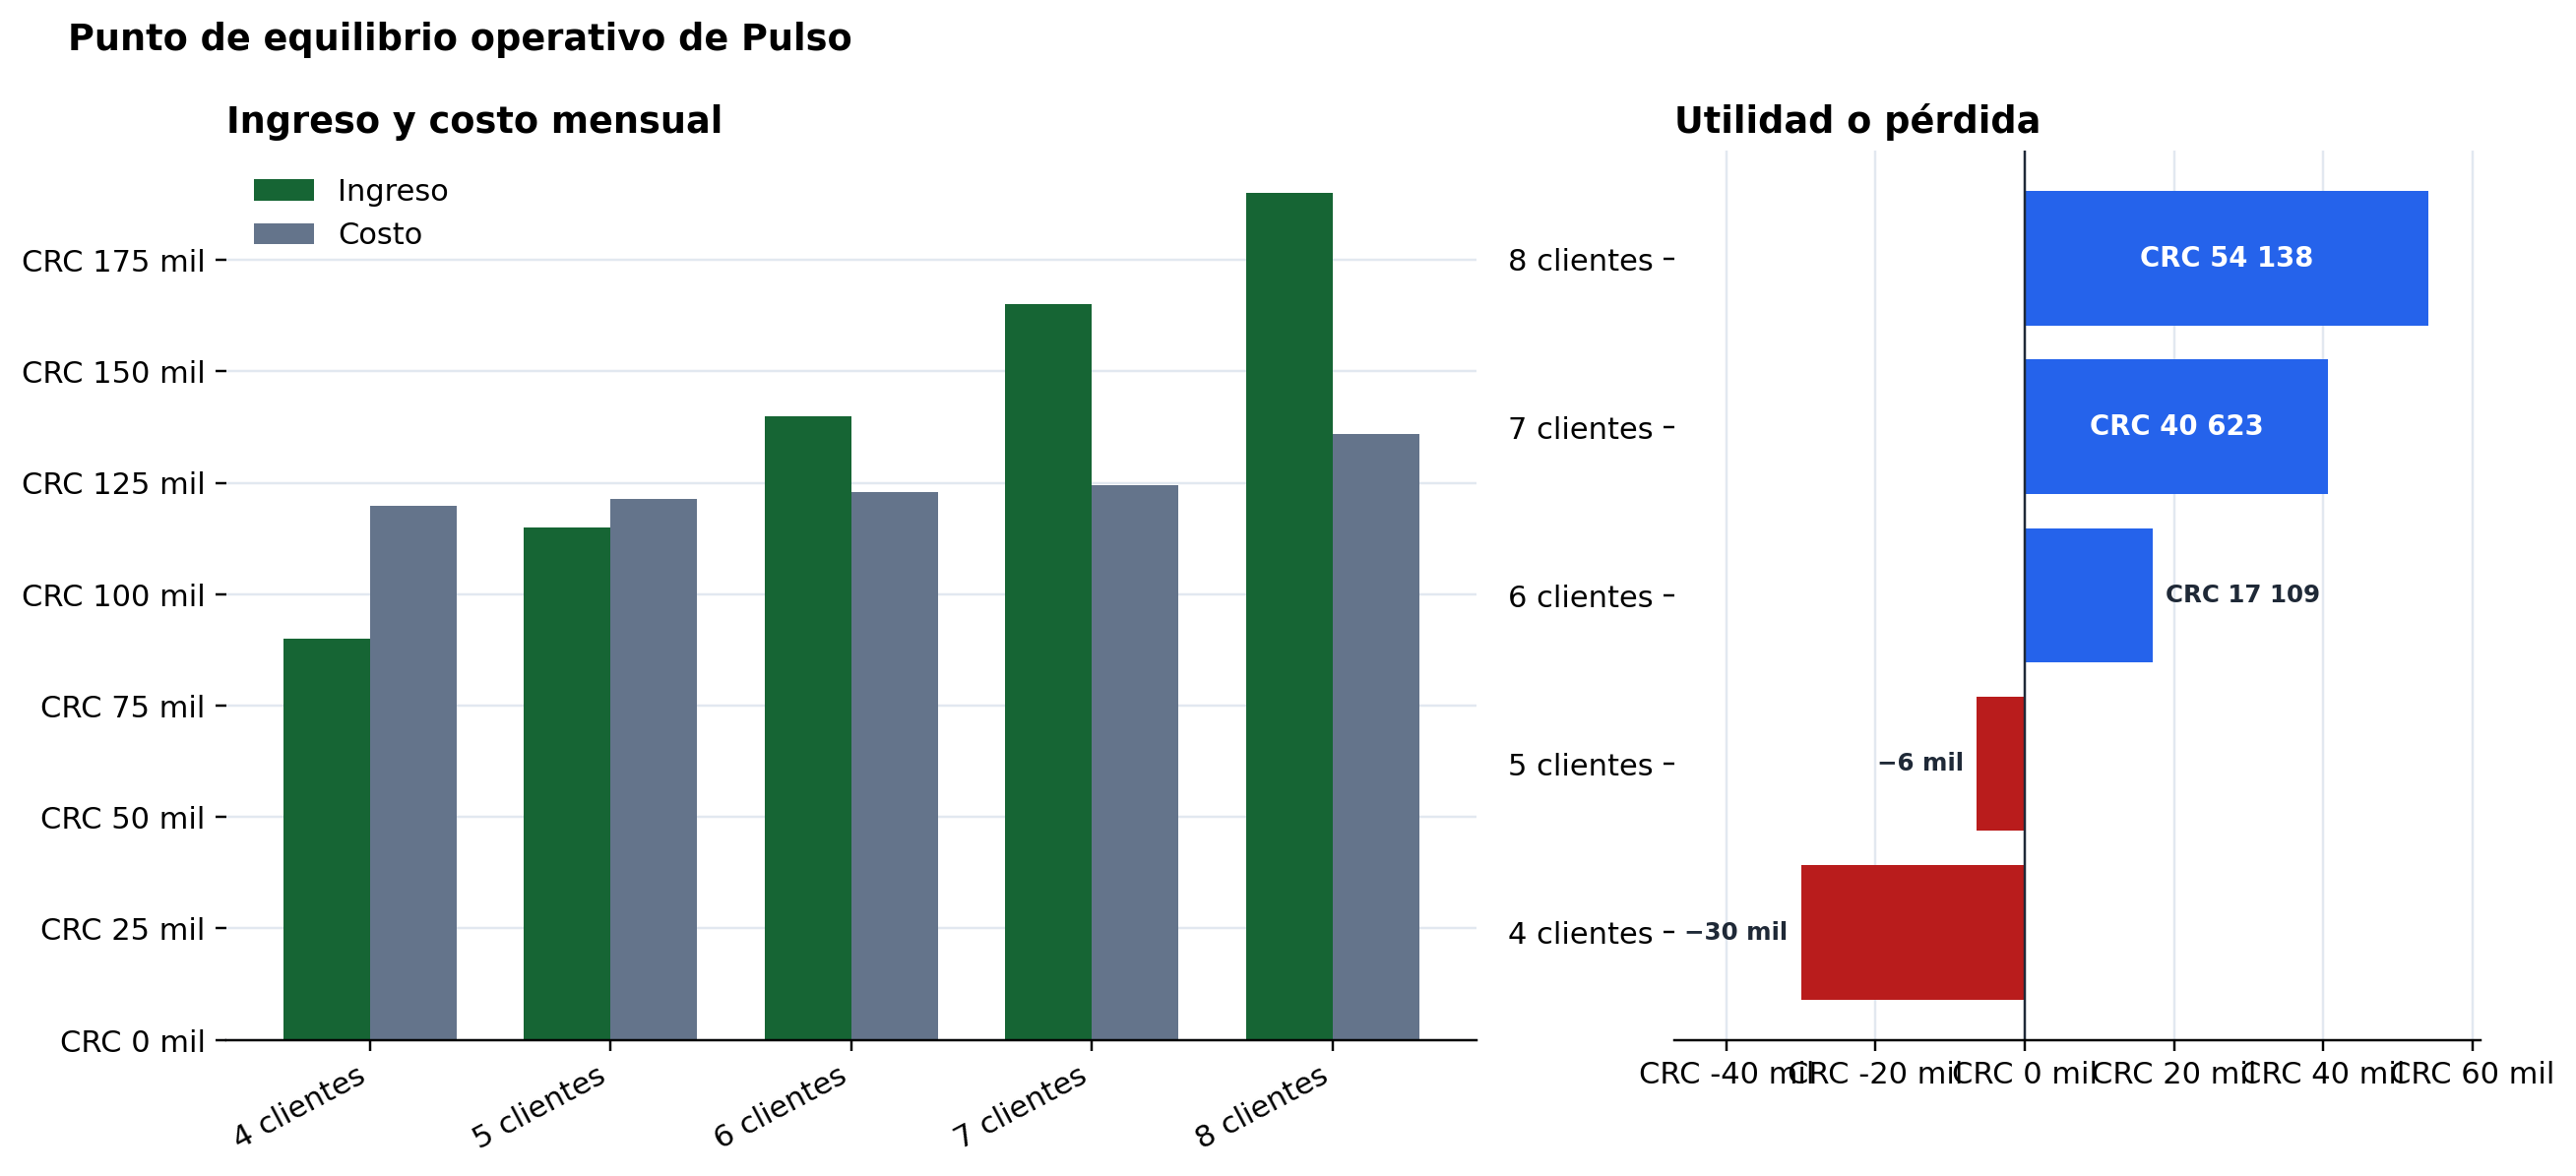
\includegraphics[width=\textwidth]{imagenes/escenarios_punto_equilibrio.png}
\caption{Punto de equilibrio operativo de Pulso}
\label{fig:escenarios-equilibrio}
\caption*{\textit{Nota}. Elaboración propia a partir del escenario financiero preliminar.}
\end{figure}

Con seis clientes se cubriría la operación mensual bajo los supuestos usados.
La recuperación del trabajo inicial se analiza por separado en la proyección
anual. El paso de cinco contrataciones iniciales a seis es parte del escenario
que termina con 14 gimnasios. Para saber si se puede alcanzar, se necesita
registrar las demostraciones, las contrataciones y la continuidad de clientes.

\subsection{Flujo de caja, sostenibilidad y seguimiento}

Cada mes se revisarán los cobros, pagos, clientes activos, cancelaciones y horas
de soporte. Si aumentan los costos, se calculará de nuevo cuántos clientes se
necesitan para cubrirlos. Aunque el resultado anual previsto es de
CRC 596\,044,36, también se debe comprobar que haya dinero disponible en las
fechas de pago.

Durante el piloto se medirá el uso, el tiempo dedicado a tareas, los problemas
y la intención de continuar. Esta información ayudará a ajustar los precios,
los gastos y el ritmo de crecimiento del servicio.

\subsection{Riesgos y medidas de respuesta}

\begin{longtable}{>{\bfseries}p{2.8cm}p{3.1cm}p{3cm}p{5cm}}
\caption{Riesgos principales del plan de negocios}\label{tab:riesgos}\\
\toprule
Riesgo & Probabilidad e impacto & Señal de control & Respuesta prevista \\
\midrule
\endfirsthead
\toprule
Riesgo & Probabilidad e impacto & Señal de control & Respuesta prevista \\
\midrule
\endhead
Pocas contrataciones & Alta; impacto alto. & Rechazos, demostraciones sin continuidad y objeciones de precio. & Registrar los motivos y revisar la oferta. \\
Aislamiento de gimnasios & Alto antes de implementarlo. & Pruebas de acceso cruzado y revisión de permisos. & No atender varios gimnasios con datos reales antes de completar la separación. \\
Consumo de nube & Medio; impacto medio. & Uso, almacenamiento, transferencia y costo mensual. & Definir límites y recalcular el equilibrio cuando cambie el consumo. \\
Soporte insuficiente & Medio; impacto medio. & Consultas pendientes, tiempo de respuesta y horas por cliente. & Mejorar las guías y revisar la carga de trabajo mensual. \\
Privacidad o seguridad & Medio; impacto alto. & Incidentes, accesos fallidos, respaldos y permisos. & Datos ficticios, mínimos privilegios, respaldo y procedimiento de respuesta. \\
Formalización legal & Alta mientras esté pendiente. & Ausencia de orientación, inscripción o cotizaciones. & Mantener carácter educativo y buscar orientación institucional y profesional. \\
\bottomrule
\caption*{\textit{Nota}. La clasificación se revisará después del piloto.}
\end{longtable}
